
%%%%%%%%%%%%%%%%%%%%%%%%%%%%%%%%%%%%%%%%%%%%%%%%%%%%%%%%%%%%%%%%%%%%%
%% This is a (brief) model paper using the achemso class
%% The document class accepts keyval options, which should include
%% the target journal and optionally the manuscript type.
%%%%%%%%%%%%%%%%%%%%%%%%%%%%%%%%%%%%%%%%%%%%%%%%%%%%%%%%%%%%%%%%%%%%%
\documentclass[journal=jacsat,manuscript=article,layout=singlecolumn]{achemso}

%%%%%%%%%%%%%%%%%%%%%%%%%%%%%%%%%%%%%%%%%%%%%%%%%%%%%%%%%%%%%%%%%%%%%
%% Place any additional packages needed here.  Only include packages
%% which are essential, to avoid problems later.
%%%%%%%%%%%%%%%%%%%%%%%%%%%%%%%%%%%%%%%%%%%%%%%%%%%%%%%%%%%%%%%%%%%%%
\usepackage{chemformula} % Formula subscripts using \ch{}
\usepackage[T1]{fontenc} % Use modern font encodings
\usepackage{epstopdf}
\usepackage{multirow}
\usepackage{adjustbox}
\usepackage{float}
\usepackage{placeins}
\usepackage{easy-todo}
\usepackage{verbatim}
%%%%%%%%%%%%%%%%%%%%%%%%%%%%%%%%%%%%%%%%%%%%%%%%%%%%%%%%%%%%%%%%%%%%%
%% If issues arise when submitting your manuscript, you may want to
%% un-comment the next line.  This provides information on the
%% version of every file you have used.
%%%%%%%%%%%%%%%%%%%%%%%%%%%%%%%%%%%%%%%%%%%%%%%%%%%%%%%%%%%%%%%%%%%%%
%%\listfiles

%%%%%%%%%%%%%%%%%%%%%%%%%%%%%%%%%%%%%%%%%%%%%%%%%%%%%%%%%%%%%%%%%%%%%
%% Place any additional macros here.  Please use \newcommand* where
%% possible, and avoid layout-changing macros (which are not used
%% when typesetting).
%%%%%%%%%%%%%%%%%%%%%%%%%%%%%%%%%%%%%%%%%%%%%%%%%%%%%%%%%%%%%%%%%%%%%
\newcommand*\mycommand[1]{\texttt{\emph{#1}}}

%%%%%%%%%%%%%%%%%%%%%%%%%%%%%%%%%%%%%%%%%%%%%%%%%%%%%%%%%%%%%%%%%%%%%
%% Meta-data block
%% ---------------
%% Each author should be given as a separate \author command.
%%
%% Corresponding authors should have an e-mail given after the author
%% name as an \email command. Phone and fax numbers can be given
%% using \phone and \fax, respectively; this information is optional.
%%
%% The affiliation of authors is given after the authors; each
%% \affiliation command applies to all preceding authors not already
%% assigned an affiliation.
%%
%% The affiliation takes an option argument for the short name.  This
%% will typically be something like "University of Somewhere".
%%
%% The \altaffiliation macro should be used for new address, etc.
%% On the other hand, \alsoaffiliation is used on a per author basis
%% when authors are associated with multiple institutions.
%%%%%%%%%%%%%%%%%%%%%%%%%%%%%%%%%%%%%%%%%%%%%%%%%%%%%%%%%%%%%%%%%%%%%

\author{Hanne Antila}
\author{Batuhan Kav}
\affiliation{Forschungszentrum Juelich, Germany}
\email{batuhankav@gmail.com}
\author{Markus S. Miettinen}
\author{O. H. Samuli Ollila}

%%%%%%%%%%%%%%%%%%%%%%%%%%%%%%%%%%%%%%%%%%%%%%%%%%%%%%%%%%%%%%%%%%%%%
%% The document title should be given as usual. Some journals require
%% a running title from the author: this should be supplied as an
%% optional argument to \title.
%%%%%%%%%%%%%%%%%%%%%%%%%%%%%%%%%%%%%%%%%%%%%%%%%%%%%%%%%%%%%%%%%%%%%
%\title[An \textsf{achemso} demo]
%  {A demonstration of the \textsf{achemso} \LaTeX\
%   class\footnote{A footnote for the title}}
\title{NMRLipids VI: Polarizable Force Fields}

%%%%%%%%%%%%%%%%%%%%%%%%%%%%%%%%%%%%%%%%%%%%%%%%%%%%%%%%%%%%%%%%%%%%%
%% Some journals require a list of abbreviations or keywords to be
%% supplied. These should be set up here, and will be printed after
%% the title and author information, if needed.
%%%%%%%%%%%%%%%%%%%%%%%%%%%%%%%%%%%%%%%%%%%%%%%%%%%%%%%%%%%%%%%%%%%%%
%\abbreviations{IR,NMR,UV}
%\keywords{American Chemical Society, \LaTeX}

%%%%%%%%%%%%%%%%%%%%%%%%%%%%%%%%%%%%%%%%%%%%%%%%%%%%%%%%%%%%%%%%%%%%%
%% The manuscript does not need to include \maketitle, which is
%% executed automatically.
%%%%%%%%%%%%%%%%%%%%%%%%%%%%%%%%%%%%%%%%%%%%%%%%%%%%%%%%%%%%%%%%%%%%%
\begin{document}

%%%%%%%%%%%%%%%%%%%%%%%%%%%%%%%%%%%%%%%%%%%%%%%%%%%%%%%%%%%%%%%%%%%%%
%% The "tocentry" environment can be used to create an entry for the
%% graphical table of contents. It is given here as some journals
%% require that it is printed as part of the abstract page. It will
%% be automatically moved as appropriate.
%%%%%%%%%%%%%%%%%%%%%%%%%%%%%%%%%%%%%%%%%%%%%%%%%%%%%%%%%%%%%%%%%%%%%
%\begin{tocentry}

%\end{tocentry}

%%%%%%%%%%%%%%%%%%%%%%%%%%%%%%%%%%%%%%%%%%%%%%%%%%%%%%%%%%%%%%%%%%%%%
%% The abstract environment will automatically gobble the contents
%% if an abstract is not used by the target journal.
%%%%%%%%%%%%%%%%%%%%%%%%%%%%%%%%%%%%%%%%%%%%%%%%%%%%%%%%%%%%%%%%%%%%%
\begin{abstract}
	
	For the initial project description, please refer to \\ https://github.com/batukav/NMRlipidsVIpolarizableFFs/blob/master/Manuscript/manuscript.pdf
	
\end{abstract}

%%%%%%%%%%%%%%%%%%%%%%%%%%%%%%%%%%%%%%%%%%%%%%%%%%%%%%%%%%%%%%%%%%%%%
%% Start the main part of the manuscript here.
%%%%%%%%%%%%%%%%%%%%%%%%%%%%%%%%%%%%%%%%%%%%%%%%%%%%%%%%%%%%%%%%%%%%%
\section{Introduction}

\textcolor{red}{some ideas for the intro/conclusion: 1) amoeba and drude are mostly used for transmembrane protein simulations. https://pubs.acs.org/doi/abs/10.1021/acsnano.1c06443 https://www.sciencedirect.com/science/article/abs/pii/S0959440X2100110X https://pubs.rsc.org/en/content/articlehtml/2021/sc/d1sc01887f etc. Validation/comparison of these simulations with the experiments are done for the proteins, not the lipids. Now since we know that the lipid dynamics and conformations are not very correct with the polarizable force fields, can these affect the protein conformations? is there a way to possibly connect this to the previous nmrlipids jacs paper?\\
}

Conventional classical molecular dynamics (MD) simulations only consider electrostatics as interactions between static point charges, set by molecular dynamics models (force fields) as an input in the beginning of the simulation. The dynamic effects arising from polarizability are ignored or at most enter the simulations in an averaged fashion in the force field parametrization process. However, since decades work~\cite{Thole1981,ando2001stable,Grossfield2003,
lamoreux2003,Antila2013 ,Lemkul2016, baker2015polarizable,jing2019polarizable } has been underway to make MD simulations explicitly polarizable in the hopes of reaching a more accurate description of the system. 

In the case of biomembranes (lipid bilayers), specifically, the molecular (dielectric) environment varies dramatically while crossing the membrane from the water phase across the dipolar/charged headgroup interface to the hydrophobic tail region. Including explicit polarizability in biomembrane modelling has the potential to provide more accurate description of membrane binding, membrane crossing, and behaviour and interactions of molecules residing within membranes, such as membrane protein folding. There certainly is room for improvement: efforts from the NMRlipids open science community have shown that the current non-polarizable lipid models cannot correctly reproduce the conformational ensemble~\cite{Botan2015,Antila2019}, conformational dynamics~\cite{Antila2021}, or ion biding~\cite{Catte2016} within MD simulations. 

Historically, there has been three main approaches to modelling polarizability: 1) the induced point dipole/multipole model where polarizable point dipoles are placed on chosen sites on a molecule, 2) the classical Drude oscillator model where polarization is modelled by separating a core and a shell charge with a spring which stretches according to the enviroment giving the site a dipole moment, and 3) the electronegativity equilization (fluctuating charge) model where atomic charges are no longer constant but can change according to the electronegativities of the molecule atoms and the electric fields from the molecular enviroment. In lipid modelling, the first two have surpassed the third in popularity. All of these approaches result in an increasing computational cost, e.g, by introducing new types of interactions, more interactions sites, or by requiring a shorter time step in the simulations.


%To avoid polarizability catastrophe where two closeby polarizable sites feed off from each other and the dipole moments grow infinitely



Considering the growing popularity of both implicitly and explicitly polarizable force fields and the increased computational cost that they require, a systematic benchmark study on polarizable force field quality is in great need. The few published studies reviewing the state of polarizable force fields for biomolecule simulations did not go beyond citing results from the existing studies~\cite{inakollu2020polarisable,jing2019polarizable,baker2015polarizable}. Recent publications show that \textit{implicit} inclusion of polarizability improves cation binding simulations when evaluated against NMR data~\cite{Melcr:2018a, melcr2019improved}, which suggest that including polarization explicitly could result in better description of ion binding as well. 
Currently, there are three main polarizable lipid force fields with explicit electronic polarization: CHARMM-Drude~\cite{li2017drude}, AMOEBA~\cite{chu2018anionicpolarizable,chu2018polarizable}, and CHARMM-Fluctuating Charge (FQ)~\cite{lucas2012charge}. 
Here we evaluate the performance of two actively developed polarizable force fields with lipid parameters available, CHARMM-Drude~\cite{li2017drude} and AMOEBA~\cite{chu2018anionicpolarizable,chu2018polarizable}, against NMR data. We use NMR order parameters to evaluate  structural properties and cation binding, whereas NMR relaxation rates and correlation times are utilized to benchmark the lipid conformational dynamics. Small angle scattering (SAXS) data is used to estimate the description of electron density profile of the membrane. Furthermore, we compare the results to the best performing non-polarizable simulations from the NMRlipids Databank\cite{Databank}.


This project has been performed within the NMRLipids collaboration (https://databank.nmrlipids.fi/)~\cite{Databank}. All simulation data, analysis scripts, and results are publicly available in their corresponding links. No plausible nor implausible request is required to download, use, and disseminate the data. 




\section{Results and Discussion}

\subsection{Evaluation of lipid bilayer properties simulated with polarizable force fields}

We start by exploring the performance of polarizable force fields using the quality metrics developed in the NMRlipids Databank (https://databank.nmrlipids.fi/)~\cite{Databank}---a quality evaluated databank for lipid simulations. These metrics describe the ability of the models to reproduce the C-H NMR order parameters (quantifying the conformations) and the SAXS data (measuring the electron density variation across the membrane). For the former the molecule is divided into three parts, one containing the headgroup and the glycerol backbone carbons and one for each of the carbonyl tails, and the quality of each is evaluated separately. The quality metrics are summarized in Table~\ref{tab:my_label} and the performance of the force fields is visualized along with the underlying experimental measurables in Fig~\ref{fig:order_parameters}. 

One can clearly see that the non-polarizable force fields, CHARMM36 and OPLS3e, consistently outperform the polarizable force fields with respect to the NMR measurables for all parts of the molecule (higher $P$-values). For older CHARMM-Drude force field, this is likely due to the headgroup and glycerol parametrization having been done targetting absolute average values of the order parameters instead of taking account the potential order parameter forking ( measurably different order parameters for different C--H bods at one carbon) and order parameter sign~\cite{Antila2022}. This was then remedied in the newer version of the model, which also provides better description of the carbon tails. In fact, for POPE sn-2 tail the CHARMM-Drude2023 gives the best description of the models investigated here.  The AMOEBA force field reproduces the most of the headgroup order parameters well for both DOPC and POPE but vastly overestimates one of the g$_3$ values, resulting in too large forking of oder parameters in this particular carbon. AMOEBA also clearly struggles to depict the tail conformations, in particular in the double bond region of DOPC (Fig.~\ref{fig:order_parameters}). In the tail regions, the CHARMM-Drude2023 appears to be the best out of the polarizable models. 

The higher $FFq$ values (Table~\ref{tab:my_label}) of the polarizable force fields for POPC indicate that they are not able to reproduce the SAXS data quite as well as the best non-polarizable force field, OPLS3e. That said, CHARMM-Drude2023, in particular, is clearly better than its non-polarizable counterpart CHARMM36 and the best out of all the models here in capturing the POPE SAXS data. AMOEBA, on the other hand, captures the SAXS profile of POPE very poorly (Table~\ref{tab:my_label} and Fig.~\ref{fig:order_parameters}D top) which is likely connected to the overall description of the lipid tails in the force fields. Note that owing the simulation size dependency of the SAXS data~\cite{Databank} one should focus on the extrema $q_{z}$[\AA$^{-1}$] when comparing the simulated and experimental data. In particular $FFq$ only measures the difference between the first minima of the simulated and experimental curves. Also note, that the method for estimating the charge density of bilayers from the simulations places electrons as point charges at the atom centers in the system and does not consider any redistribution of charge density due to the polarizability. Nevertheless, we expect this results into a good estimate of the charge density for the calculation of the SAXS curve.

\subsection{Evaluation of conformational dynamics of lipids}

We proceed to evaluate (Fig.~\ref{fig:correlation_times}) the structural dynamics of the polarizable models againts NMR $R_{1}$ rates, here measured at a magnetic frequency that captures a window of dynamics around $\sim$0.1-1~ns, and effective correlation times $\tau_{\mathrm{eff}}$ which quantifies a larger range of dynamical processes up to $\sim$1000~ns. We include the same measurables calculated from non-polarizable CHARMM36 and SLipids force fields---the best MD force fields regarding the dynamics~\cite{Antila2021}---as a point of comparison. The AMOEBA force field captures the dynamics with respect to both measurables very well,  in par with the best non-polarizable models. In contrast, the dynamics of CHARMM-Drude appears to be faulty in the fast range ($R_{1}$ rates) and, furthermore, $\tau_{\mathrm{eff}}$ values reveal vastly too slow overall dynamics. The updated CHARMM-Drude2023 does not significantly improve the dynamics at the fast range investigated here. The effective correlation times of the newer Drude model are improved but still an order of magnitude too slow. This indicates that not only are the simulations with this polarizable force field computationally costly but one would have to simulate longer to obtain converged results. The non-polarizable counterpart of the Drude model, CHARMM36, exhibits much more realistic, faster effective correlation times. Interestingly, it has also been observed that CHARMM-Drude models have slower dynamic of water hydrogen bonding around amino acids compared to their non-polarizable counterpart~\cite{Ngo2019} which might align with an overall slower dynamics of the model in addition to enhanced water binding. Note that the experimental data here is from POPC. However, chemically identical the headgroup region the dynamics is assumed to be practically identical in DOPC, due to the decoupling of the dynamics between the headgroup and the glycerol regions~\cite{Antila2022rot, Klauda08}.

\subsection{Cation binding to membranes in polarizable simulations}

Finally, we address the premise that adding polarizability to force fields improves the depiction of ion binding to biomembranes in simulations. For this, we use the concept of "lipid electrometer"~\cite{Catte2016} where the amount of ion binding to the membrane can be quantified by the change in $\alpha$ and $\beta$ order parameters upon increasing salt concentration. These changes in order parameters are depicted in Fig.~\ref{fig:popc_order_parameter_change} whereas Fig.~\ref{fig:ion_density_profiles} gives the density profiles of ions with respect to the bilayer normal. The CHARMM-Drude2017 exhibits strong sodium binding, evidenced both by large change in the order parameters and the ion density profiles. Based on the change in the order parameters, the sodium binding is even stronger than the divalent calcium binding. In strong contrast, experimentally one sees no sodium binding and some binding of calcium ions. Too strong sodium binding in the CHARMM-Drude model has been indicated before for peptides/amino acids~\cite{Ngo2019, Kav2022} and deep-eutectic solvents~\cite{shayestehpour2022ion} along with a too strong calcium interactions~\cite{Tan2022} in line with what we observe here for the lipids. 

The faulty sodium ion binding seems to have been somewhat remedied in the CHARMM-Drude2023 force field: the change of the order parameters is diminished to be more in line with experiments and only the some accumulation of sodium ions near the phosphate oxygen is seen in the ion distributions. Based on the change in the order parameters, the calcium binding also appears to be better represented in the updated model. The ion distributions reveal that binding of calcium has moved deeper into the bilayer and there is a stronger formation of ionic double layer by subsequent attraction of chloride into the bilayer. However, this the ion layering is most prominently present in the original CHARMM36 force field, for for sodium and calcium ions. Note, that both for sodium and calcium ion additionin the CHARMM-Drude2023force field reintroduces the forking of order parameters at the $\beta$ carbon in particular. These might also be a sign of poor convergence of the simulations owing to the slow conformational dynamics detected above, which would also not be fully reflected in the calculation of error estimates for the order parameters. 

As opposed to the CHARMM36-Drude model, the order parameters of the AMOEBA model are almost completely unaffected by the ion addition, both for NaCl and CaCl$_{2}$. The ion density profiles confirm that very little ions penetrate the membrane region where the lipid phosphates reside. While this is in line with experiments regarding sodium ions, there should be some binding of calcium ions to the membrane. Again, the change in the order parameters indicate the non-polarizable CHARMM36 depicts sodium binding the best out of the models compared here, being slightly more realistic than its most recent polarizable counterpart, CHARMM-Drude2023. Regarding calcium binding, CHARMM36 captures the $\Delta^{\alpha}_{CH}$ about as well as the CHARMM-Drude2023, but the change in the $\beta$ carbon is better represented in the CHARMM-Drude2023 and AMOEBA models. This suggest that some accuracy might have been gained in modelling the divalent ion binding with polarizable models but the advantage is not clear. No force field, polarizable or non-polarizable, is able to model both monovalent and divalent ion binding flawlessly. This is of note, as polarizable force fields are often assumed superior and concequently a popupar choice in modelling, eg, ion channels~\cite{sun2017 jing2019polarizable, klesse2020induced}\todo{I think there is a mistake in the C36 data, firsly, the concentration should probably be 950mM instead of 1000mM and secondly the monovalent anion and cation curves look identical} ~\todo{batuhan: I fxed the anion and cation curves. Yes, C36 data is at 950mM but explicitly adding this as a new color could clutter the figure. Should I just mention this in the caption?}.



\begin{figure}[t]
    \centering
    %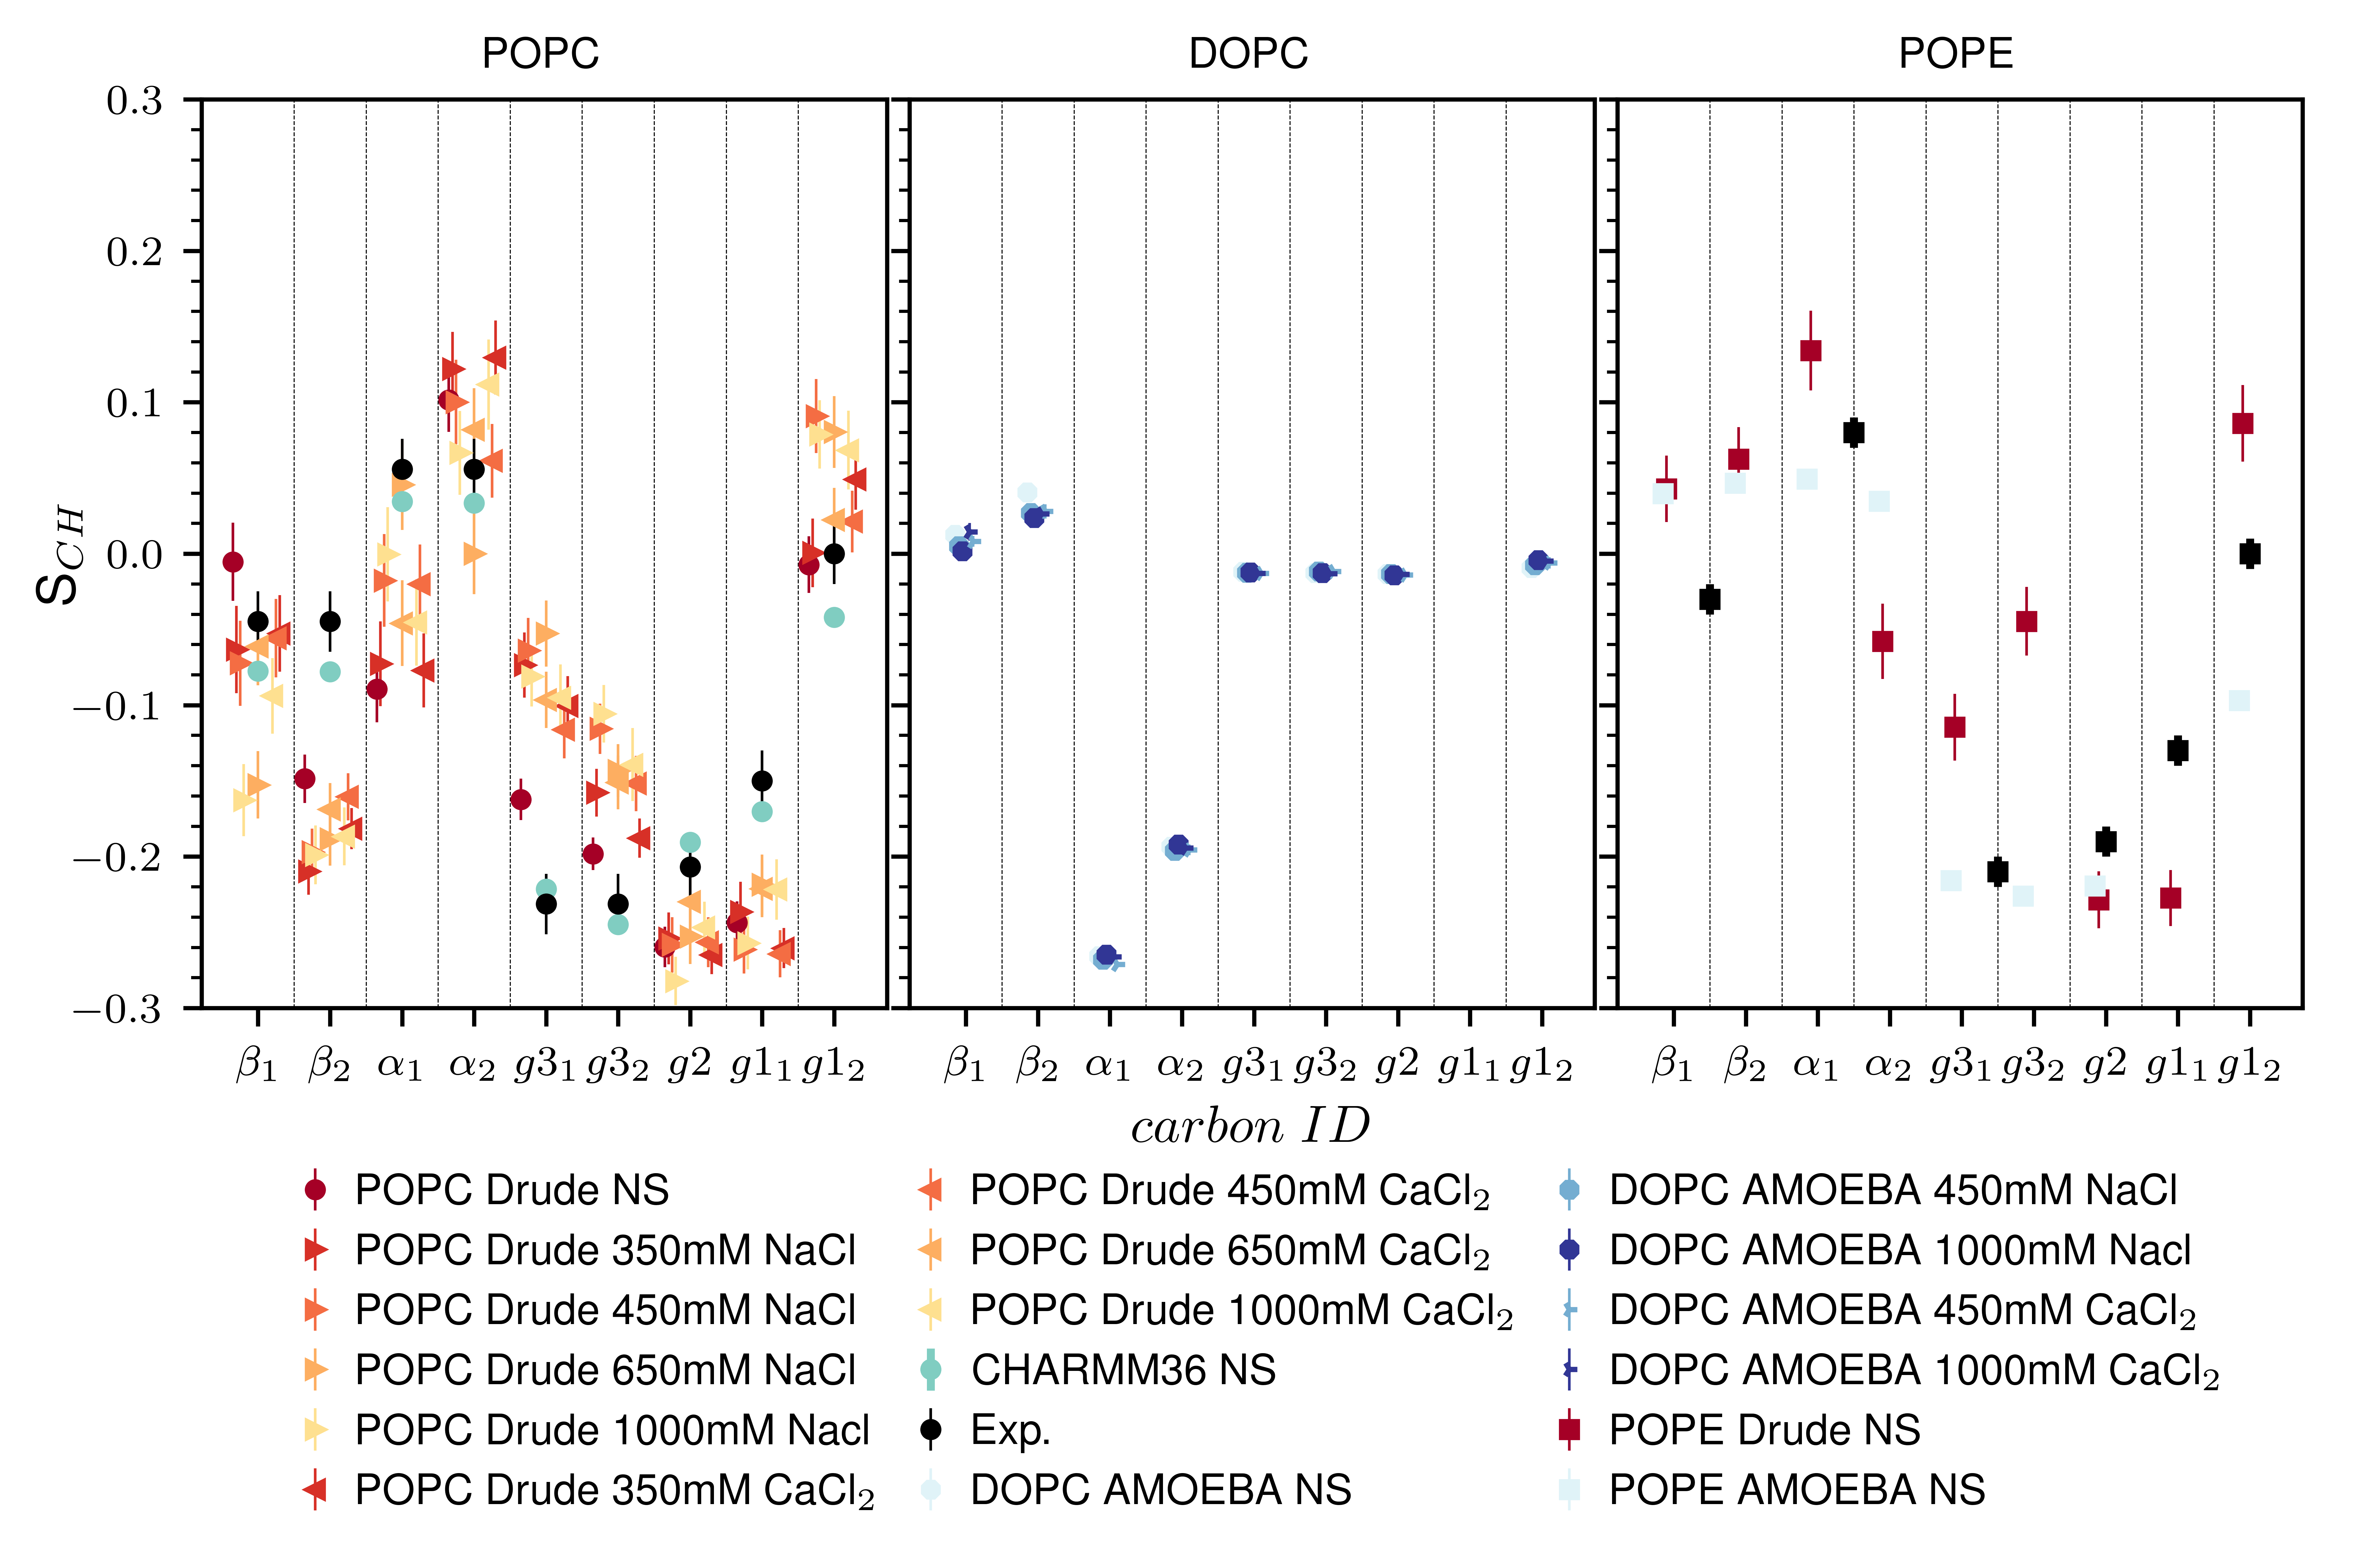
\includegraphics{Figures/order_parameters.png}
    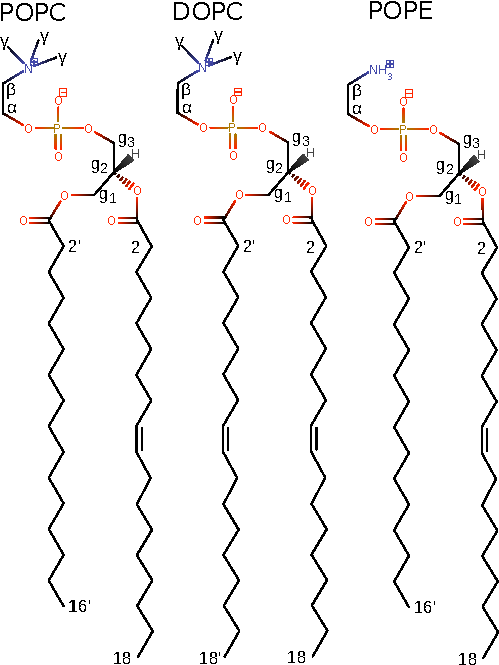
\includegraphics[width=0.4\textwidth]{Figures/molecules.pdf}
    \caption{Molecules and atom labelling used.}
    \label{fig:molecules}

\end{figure}

\begin{figure}[!hbt]
    \centering
    %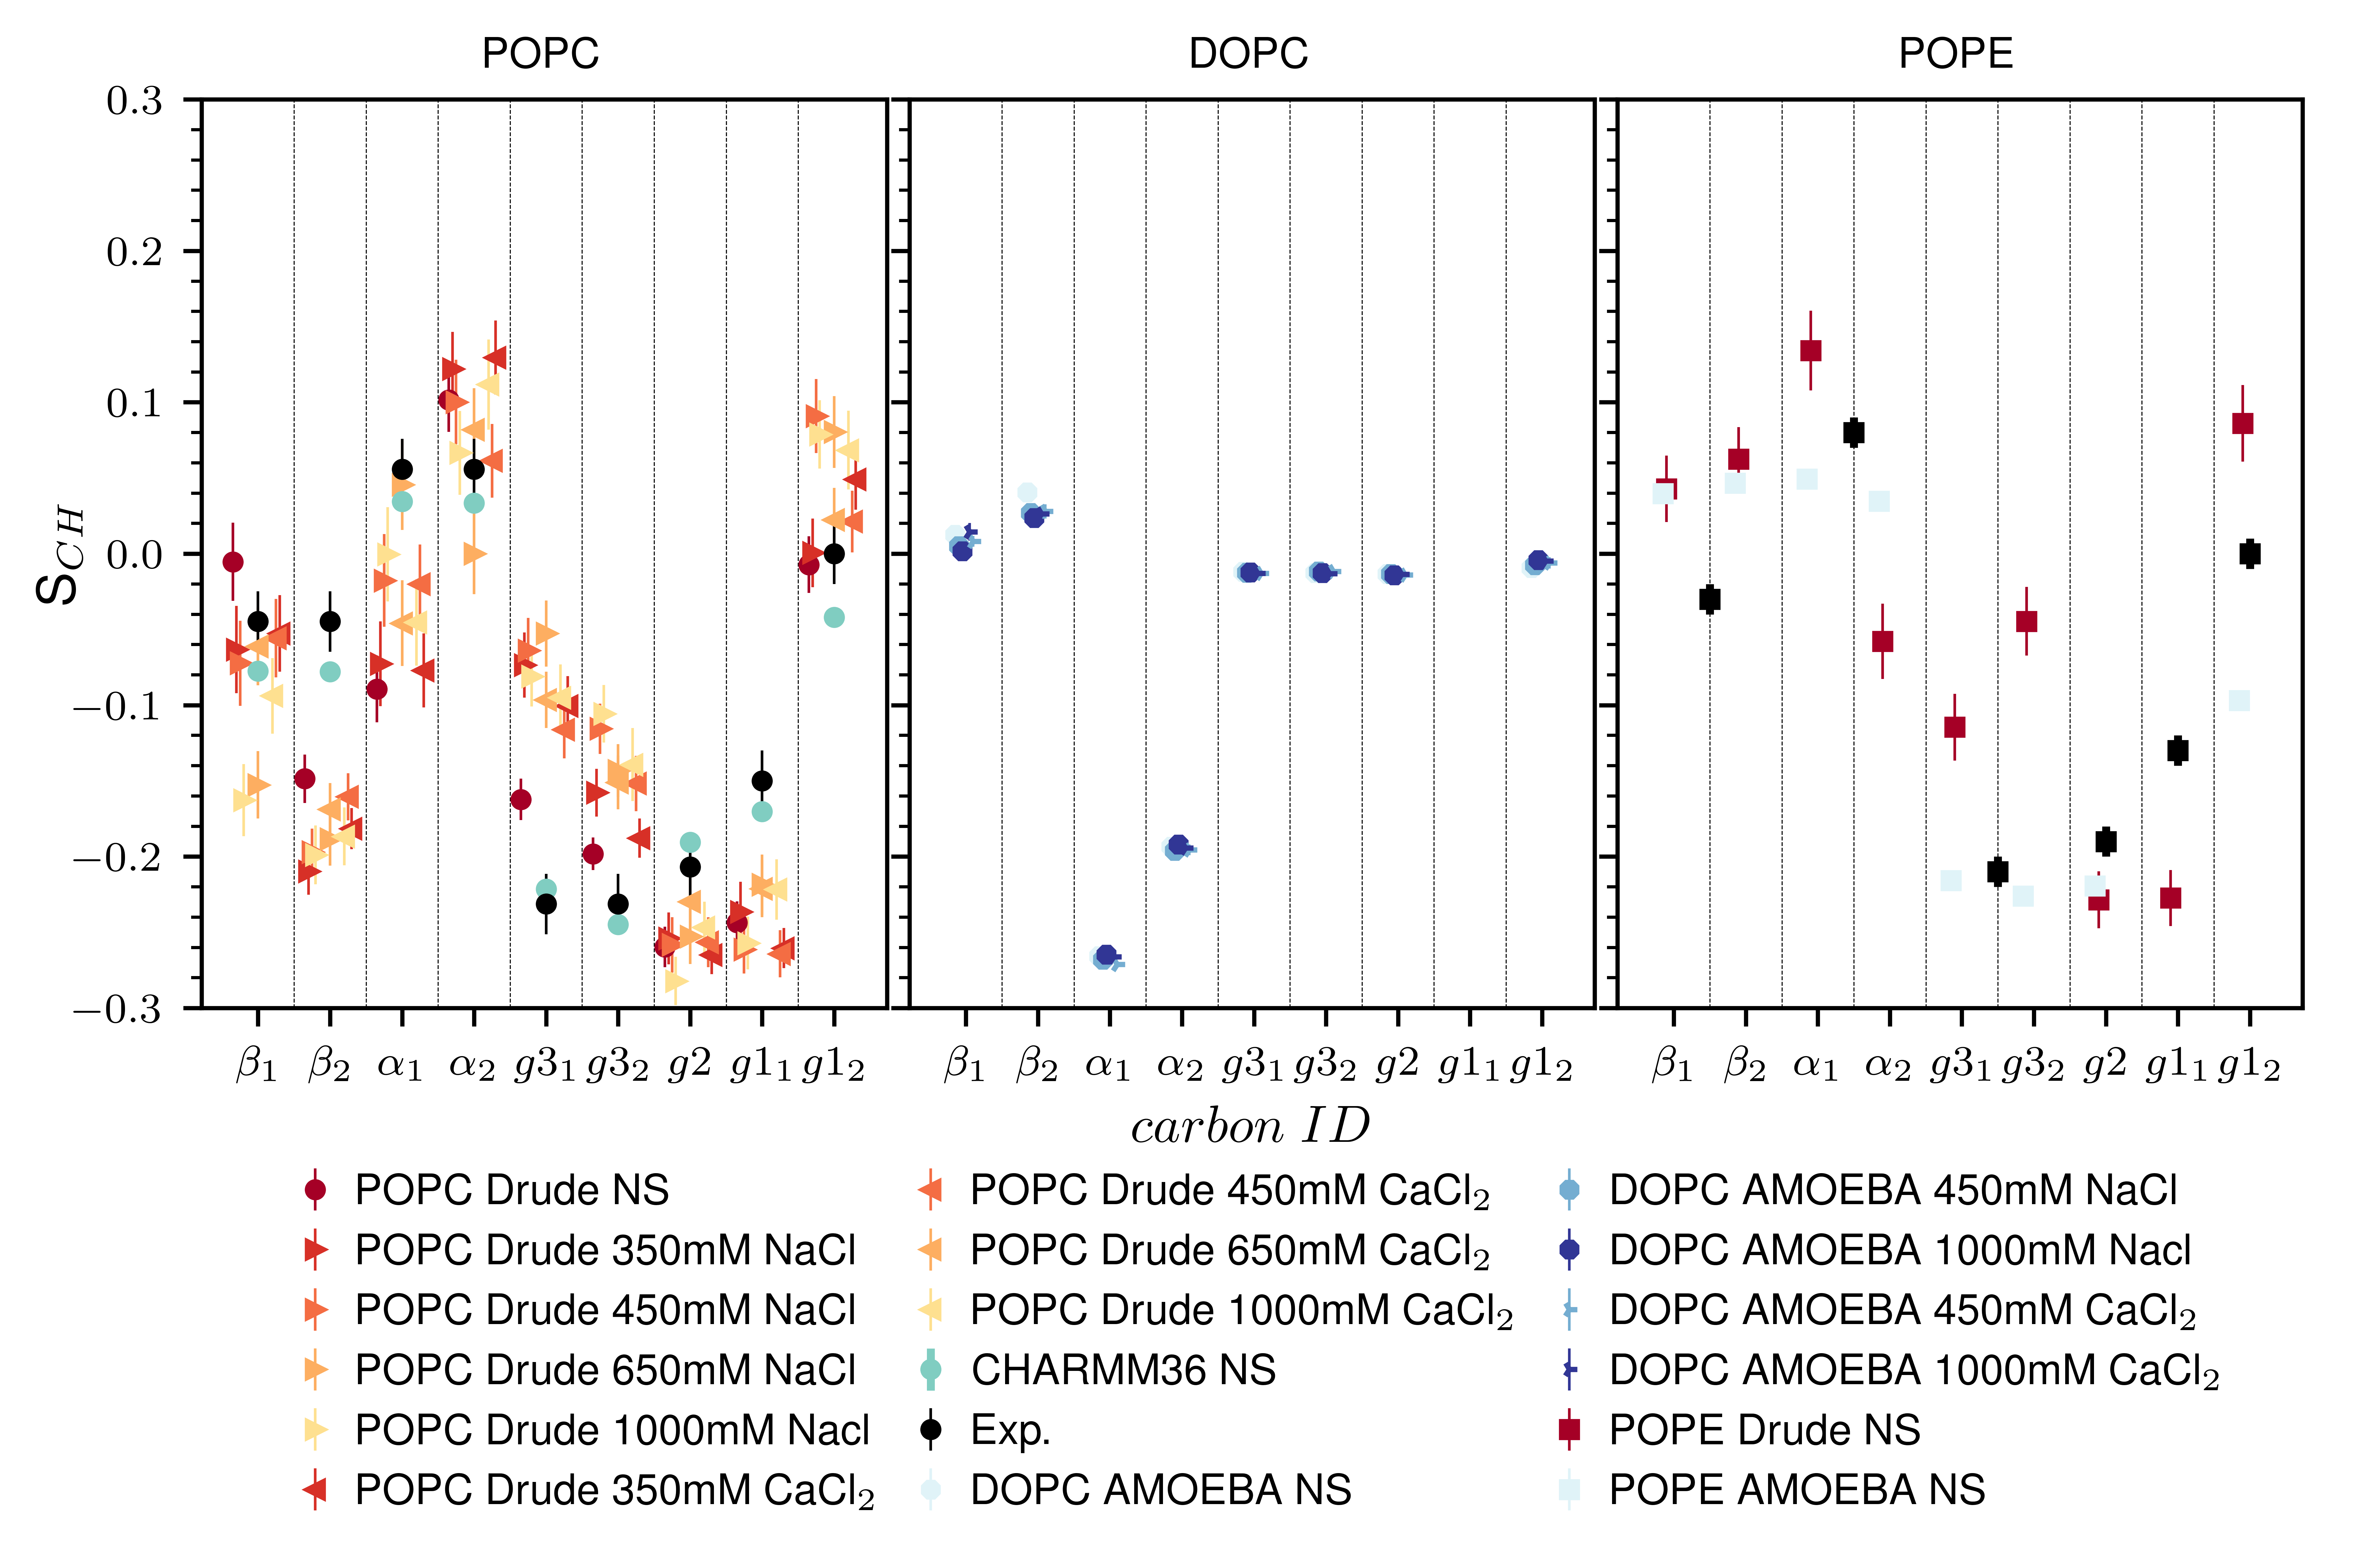
\includegraphics{Figures/order_parameters.png}
    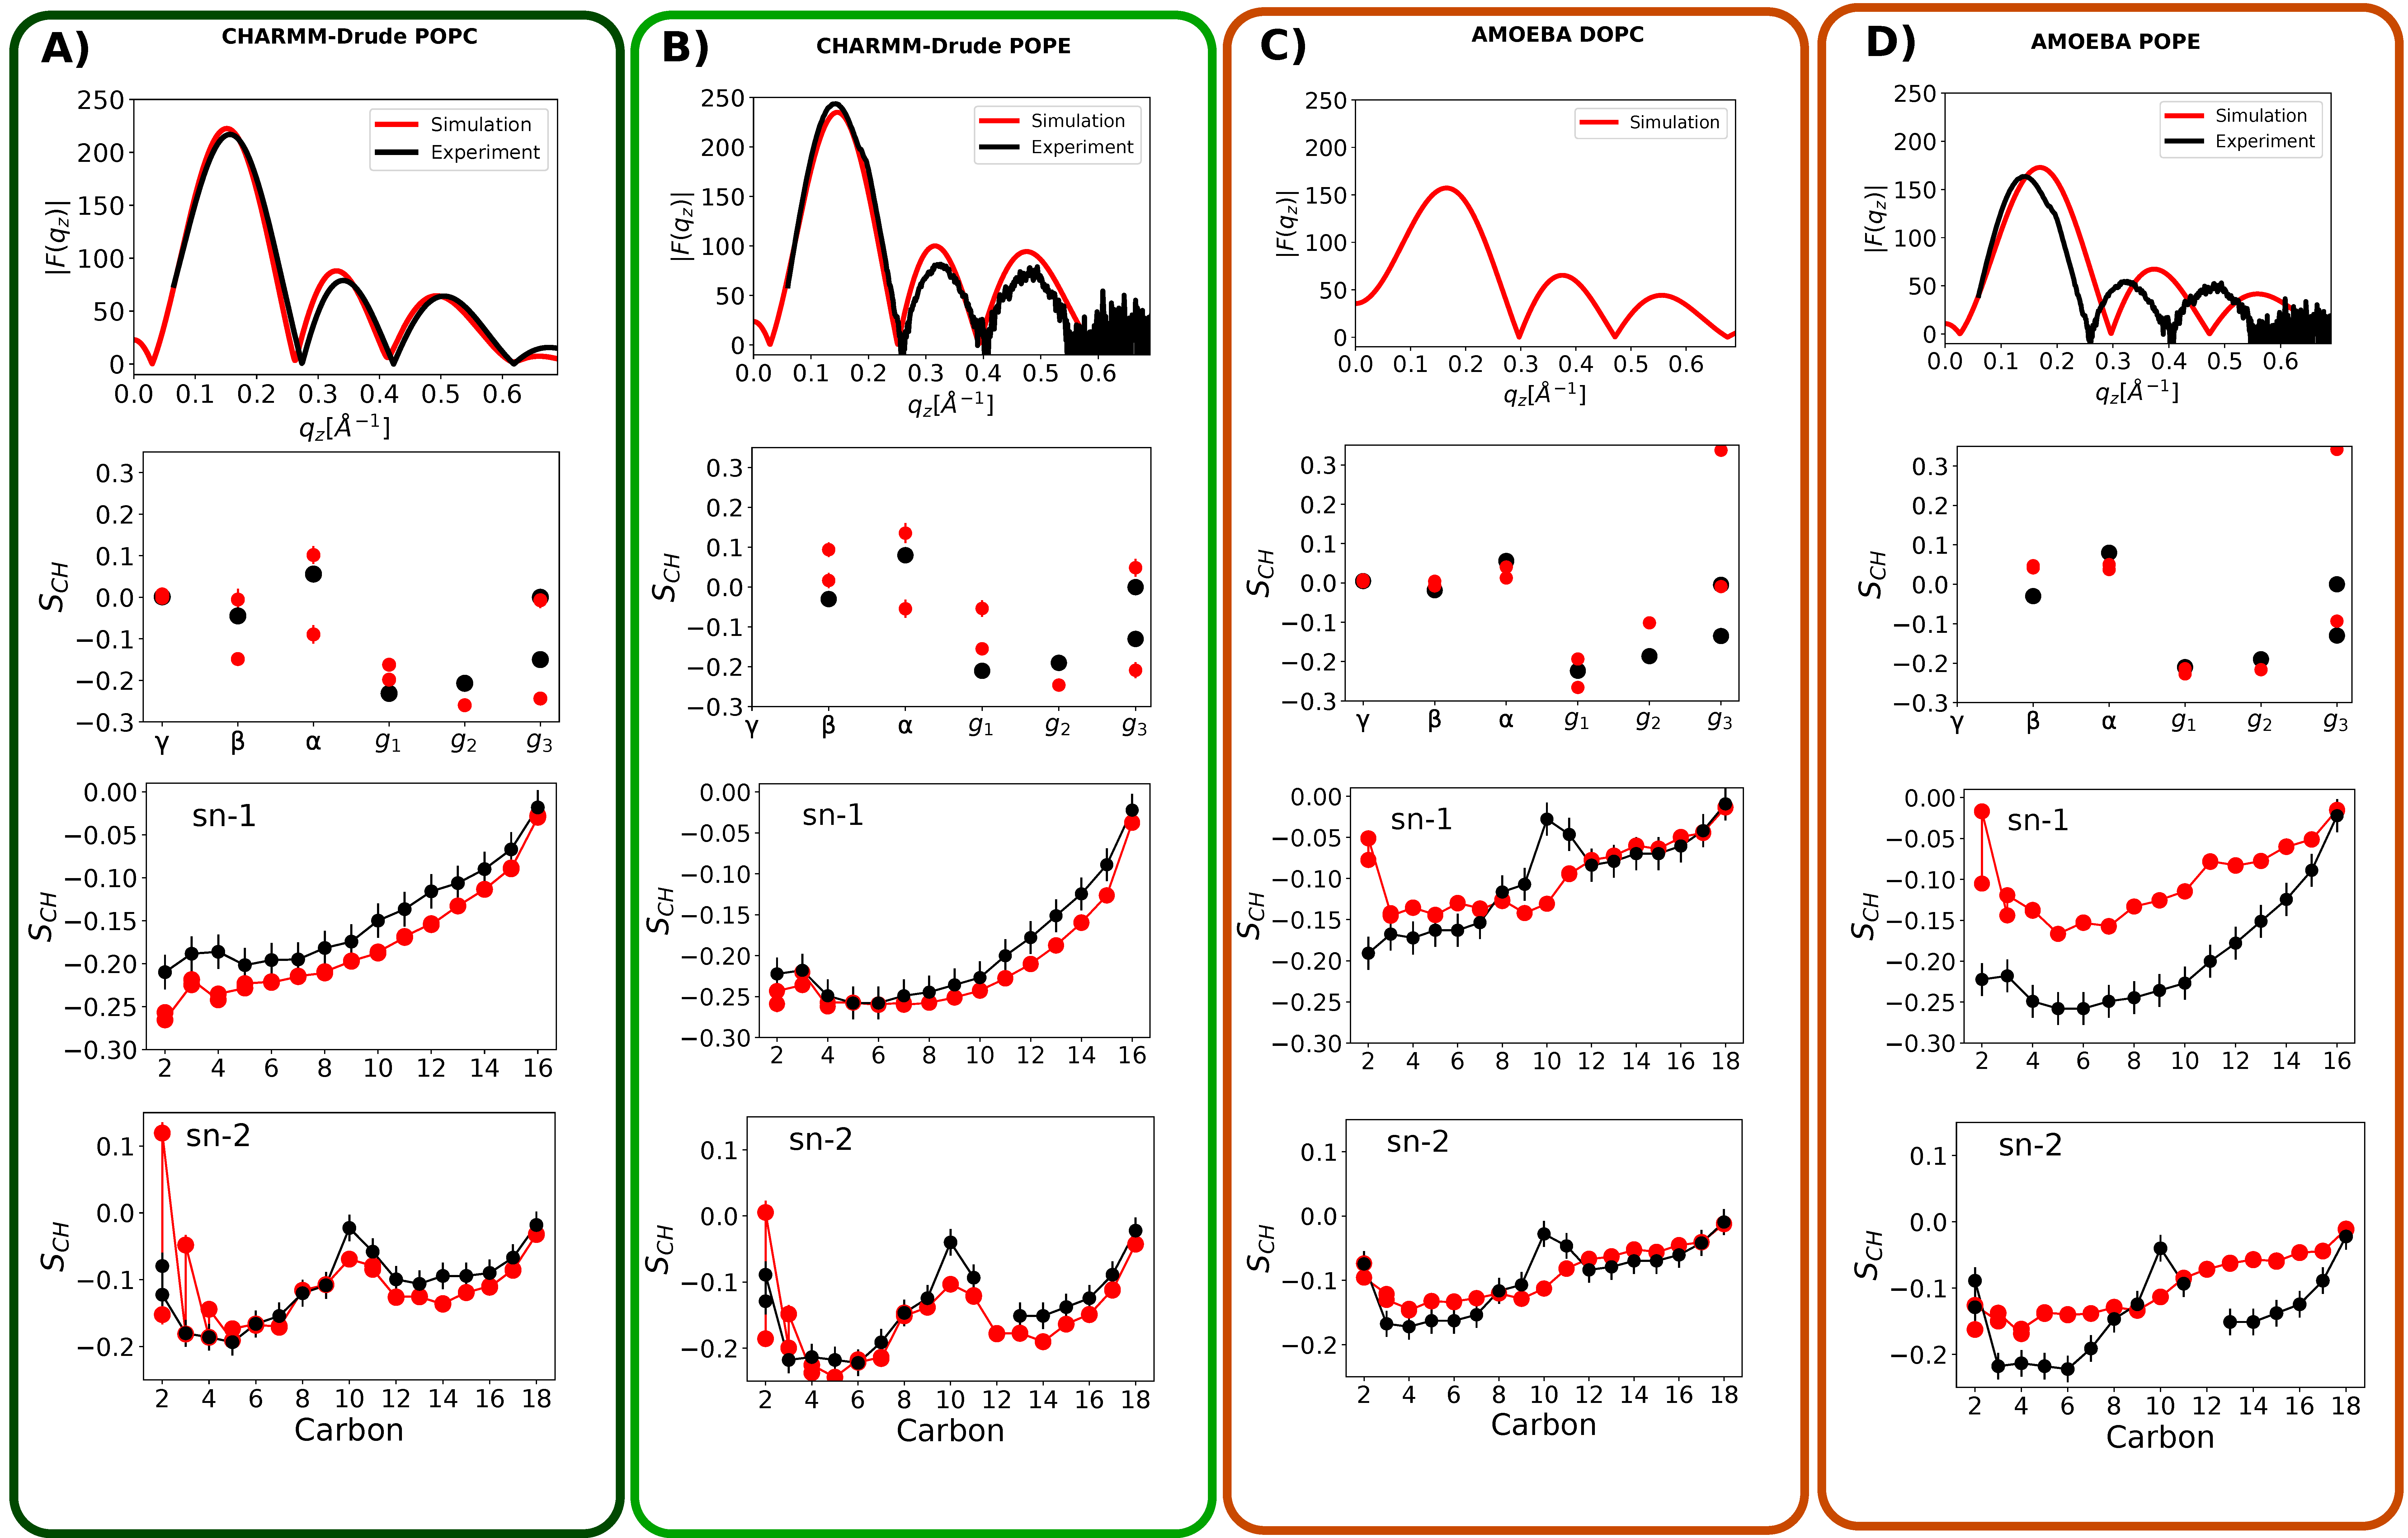
\includegraphics[width=0.8\textwidth]{Figures/quality.pdf}
    \caption{X-ray scattering form factors, and C-H bond order parameters for headgroup and glycerol backbone, and acyl chains (from top to bottom) compared between simulations and experiments using the NMRlipids databank. The atom labelling is as depicted in Fig.~\ref{fig:molecules}.}
    \label{fig:order_parameters}

\end{figure}


\begin{table}[]
    \centering
    \begin{tabular}{c c c c c c c}
        Lipid & Force field & $P^{\mathrm{headgroup}}$ & $P^{sn-1}$ & $P^{sn-2}$ & $FF_{q}$ & APL \\
        \hline
        POPC & OPLS3e       & 0.76 & 0.87 & 0.85 & 0.15 & 66.5\\
        POPC & CHARMM36     & 0.70 & 0.54 & 0.69 & 1.16 & 65.0\\
        POPC & CHARMM-Drude & 0.51 & 0.22 & 0.47 & 1.16 & 62.5\\
        POPC & CHARMM-Drude2023 & 0.50 & 0.49 & 0.53 & 0.82 & 64.5\\
        \hline
        POPE & GROMOS-CKP & 0.29 & 0.83 & 0.48 & 0.40 & 59.6\\
        POPE & CHARMM36   & 0.54 & 0.52 & 0.27 & 1.30 & 57.2 \\
        POPE & CHARMM-Drude & 0.06 & 0.53 & 0.27 & 0.80 & 56.6  \\
        POPE & CHARMM-Drude2023 & 0.28 & 0.59 & 0.54 & 0.00 & 61.4  \\
        POPE & AMOEBA & 0.21 & 0.10 & 0.23 & 3.80 & 66.9\\
        \hline
        DOPC & AMOEBA & 0.60 & 0.60 & 0.54 & - & 70.2\\
    \end{tabular}
    \caption{NMRlipids databank quality evaluations~\cite{Databank} and area per lipids compared between the best simulations found from the NMRlipids databank, simulations with CHARMM36 force field, and simulations with polarizable force fields. Experimental estimations for areas per lipid are POPC: 64.3$\pm1$\AA$^{2}$\cite{kucerka2011}, DOPC: 67.5$\pm1$\AA$^{2}$\cite{kucerka2008}, and POPE: 56.7$\pm$3\AA$^{2}$\cite{Rickeard2020}.}
    \label{tab:my_label}
\end{table}

%\begin{figure}[!hbt]
%	\centering
%	\includegraphics{dihedral_distributions_for_all.png}
%	\caption{The distributions of the torsion angles for the head group atoms}
%	\label{fig:dihedral}
%        \todo{SAMULI: I am not sure if we need this figure at all.
%          Or were you planning to discuss why order parameter response to ions is qualitatively incorrect in Drude PC?
%          If yes, then maybe remove POPE from this figure.
%        }
%\end{figure}

\begin{figure}[!hbt]
	\centering
	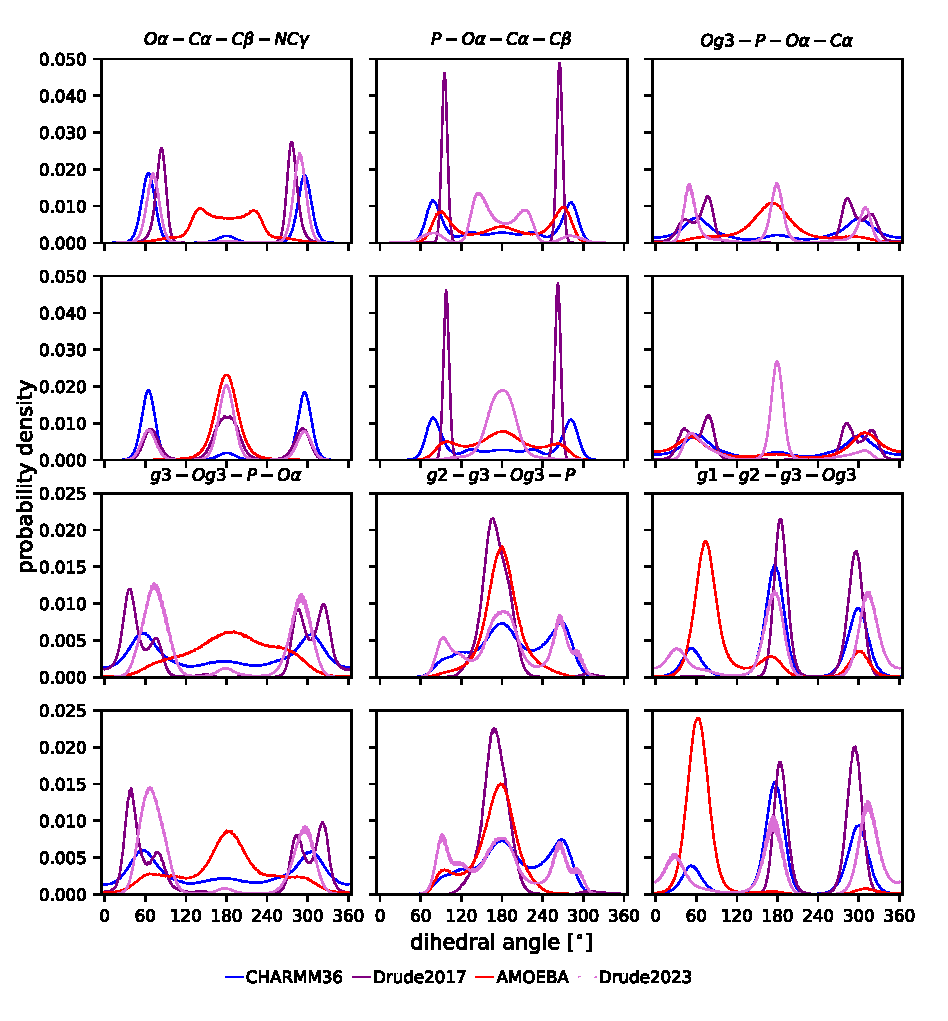
\includegraphics{Figures/dihedral_distributions_without_ions.eps}
	\caption{The distributions of the torsion angles for the head group atoms. For each torsion angle, the upper and lower rows contain the DOPC (AMOEBA) - POPC (Drude/Drude2023) and POPE lipids, respectively.}
	\label{fig:dihedral_no_salt}
\end{figure}

\begin{figure}[!hbt]
	\centering
	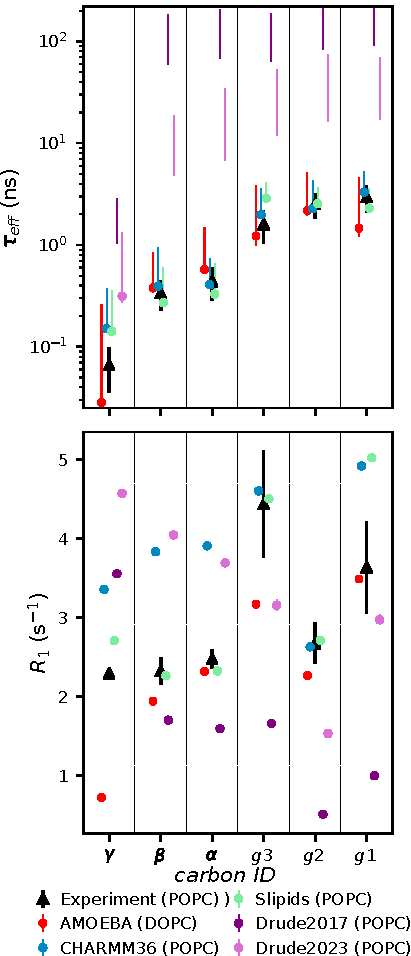
\includegraphics{Figures/both_inkscp.pdf}
	\caption{Effective correlation times (top) and R$_1$ rates (bottom) for the polarizable models and best performing non-polarizable force fields. Note, top panel axis is logarithmic to visualize the slow Drude dynamics. Experimental values are obtained from Ref.~\citenum{Antila2022rot}. All simulations used here were salt free.}
	\label{fig:correlation_times}


\end{figure}

\clearpage

\subsection{Ion binding to membranes in simulations with polarizable force fields}


\begin{figure}[!hbt]
	\centering
	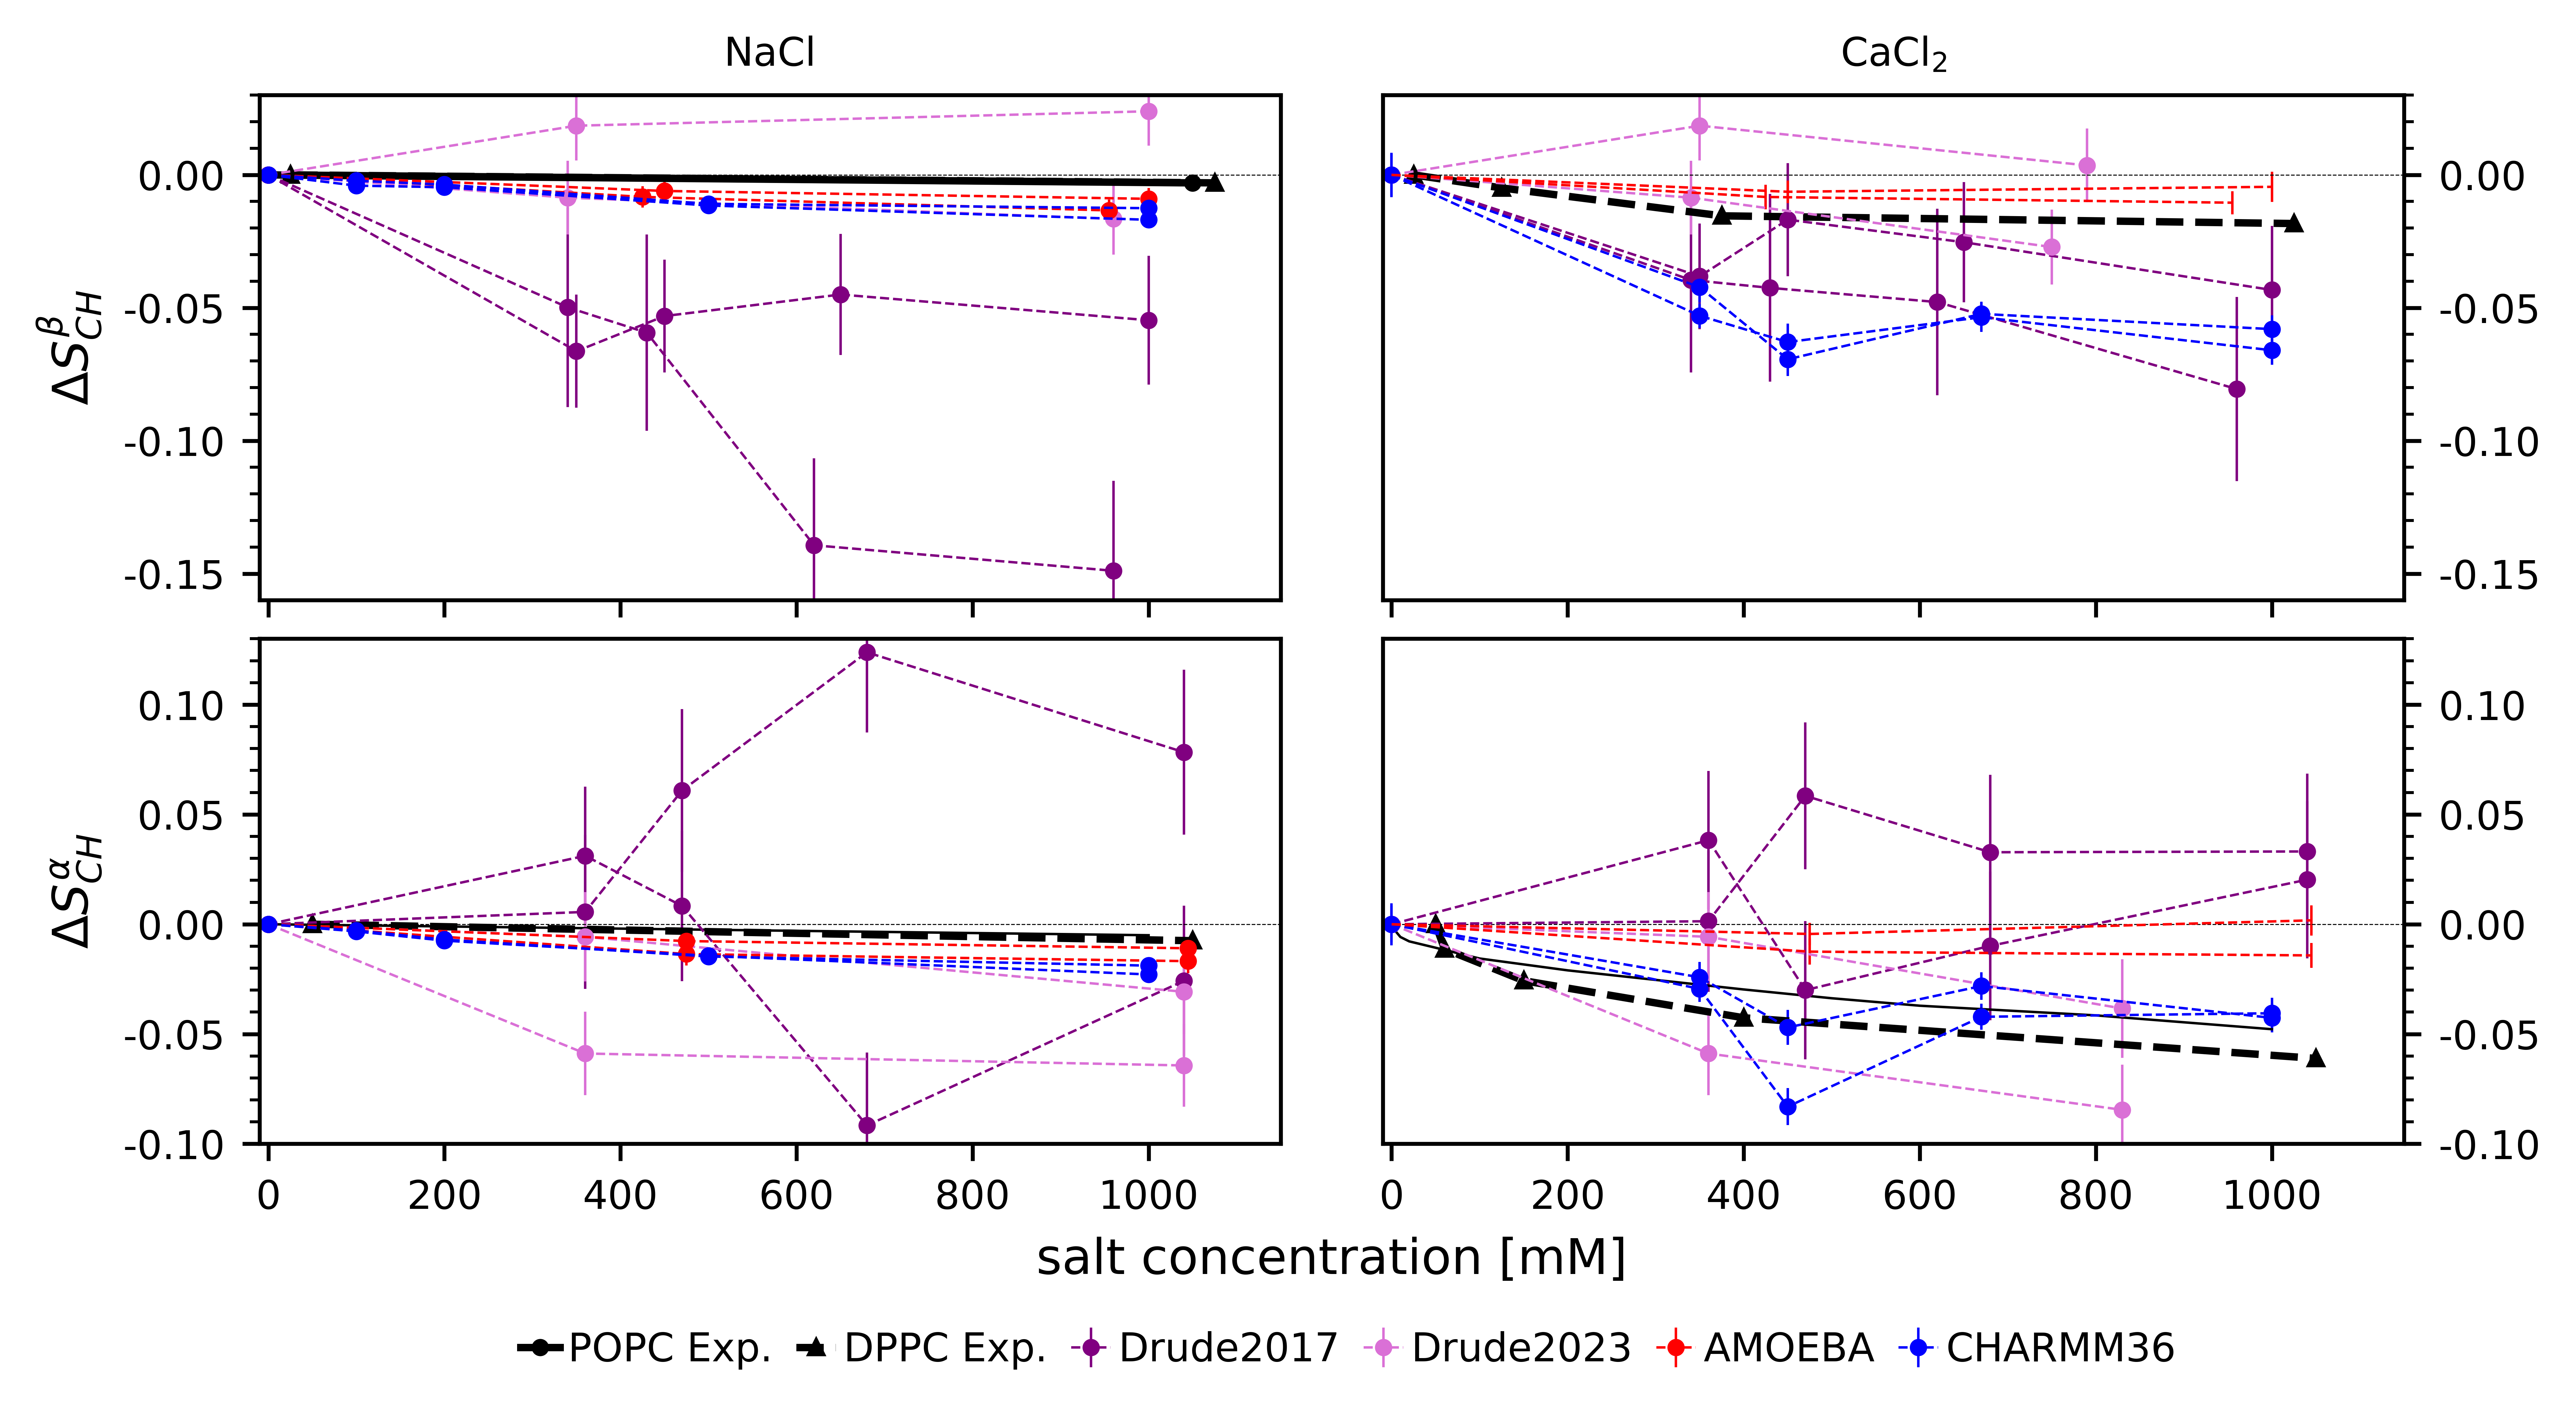
\includegraphics{Figures/order_parameter_change.png}
	\caption{The change in the lipid head group order parameters $\beta$ (top row) $\alpha$ (bottom row) upon increasing ion concentration with respect to the simulations without salt. }
	\label{fig:popc_order_parameter_change}
\end{figure}

\begin{figure}[!hbt]
    \centering
    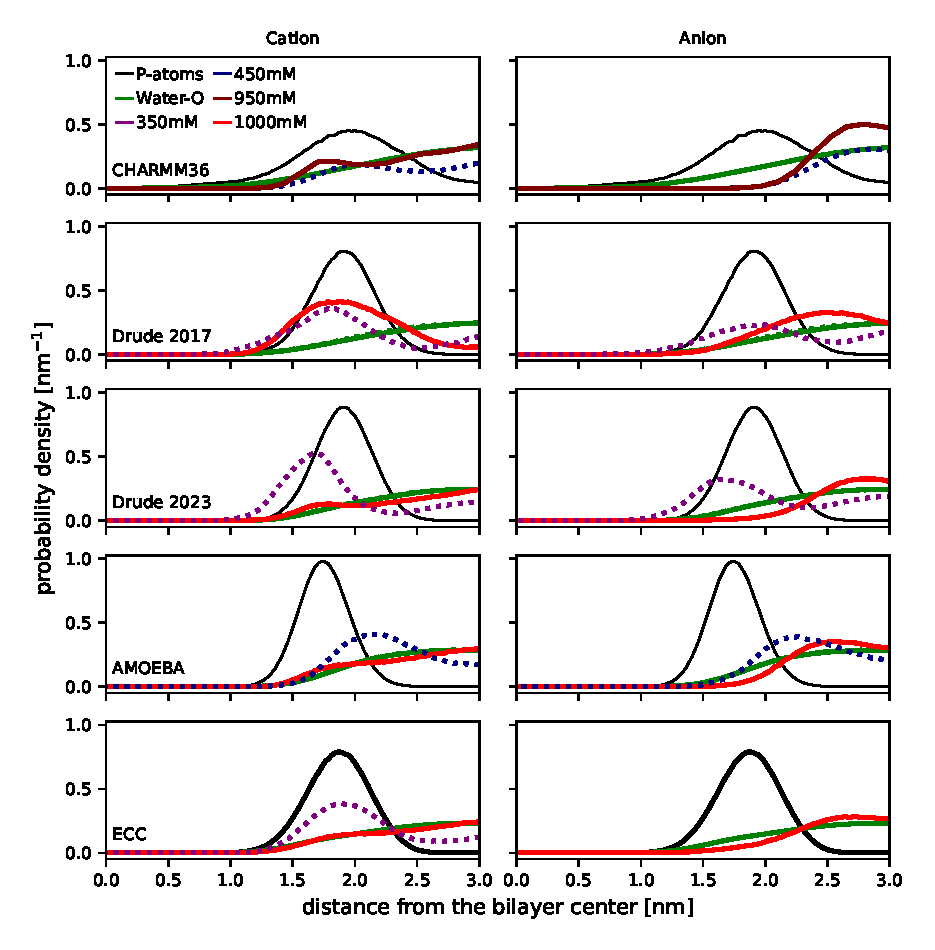
\includegraphics{Figures/ion_density_profiles_with_chloride.eps}
    \caption{Density profiles along the membrane normal for the CHARMM36 (first row)~\cite{Catte2016}, Drude 2017 and 2023 POPC (second and third rows), AMOEBA DOPC (fourth row), and electronic continuum correction (ECC, last row)~\cite{Melcr:2018a}. Solid and dashed lines are for the systems with the NaCl and CaCl$_{2}$, respectively. Please note that only 350~mM and 450~mM CaCl$_{2}$ concentrations are shown for the Drude and AMOEBA force fields, respectively, while 1000~mM NaCl concentration is shown for all force fields. CHARMM36 NaCl simulations are at 950~mM.}
    \label{fig:ion_density_profiles}
            \todo{SAMULI: We should also show the ion density profiles along membrane normal and compare the ones with 1000 mM NaCl and 350 mM CaCl$_2$
          (concentration in bulk water) to the best profiles in the literature (Fig. 5 in http://dx.doi.org/10.1021/acs.jpcb.7b12510).
          This will show the actual difference in ion binding to the best performing models available.}
          \todo{Batuhan: Data generated from http://dx.doi.org/10.1021/acs.jpcb.7b12510}
\end{figure}


\clearpage

\subsection{Discussion}

\textcolor{red}{For the ion binding discussion: drude calcium overbinds to proteins. this is known here https://pubs.acs.org/doi/full/10.1021/acsphyschemau.1c00039
drude sodium overbinds to proteins, as shown here https://pubs.rsc.org/en/content/articlepdf/2022/ra/d2ra01478e and https://onlinelibrary.wiley.com/doi/abs/10.1002/adts.201800106. Venable also cautioned us against using any ion parameters with the drude force fields. This is important as 1- polarizable force fields are supposed to be better for ion parameters and 2- they are generally used to study the ion channels.}

\subsection{Conclusions}
After comparing the polarizable lipid models against high-resolution experimental data and the best performing non-polarizable force fields, we cannot confirm that adding polarizablity to the force fields has yet solved many of the issues it was hoped to address. Monovalent ion binding is best represented in the non-polarizable CHARMM36 and the polarizable AMOEBA. However, AMOEBA does not model well the divalent ion binding to bilayers. For calcium binding the best models are CHARMM36 and the polarizable CHARMM-Drude2023.
 The electron density profiles of the bilayers are quite well captured by CHARMM-Drude2023 but rather poorly by AMOEBA, within the confines of the approximations used to calculate them from the trajectories. AMOEBA's poor performance regarding electron density curves might be related to the poor representation of lipid tail conformations in the force field, revealed by the order parameters. While CHARMM-Drude2023 captures tail and the headgroup conformations well, the non-polarizable models still outperform when comparing the order parameters. When investigating the conformational dynamics the AMOEBA force field produces results, specifically in the headgroup region of PC lipids, that are in par or better than the best non-polarizable force fields. However, the Drude models exhibit an extremely slow dynamics which leads to deficient sampling and compounding simulation time cost when using the model. In summary, the added complexity of polarizability has not still realised its potential to the fullest; The non-polarizable force fields with longer and more intense refinement behind them still outperform the polarizable models in some respects. Considering the complexity and cost of using these models, polarizability should be parameterized with more thorough consideration to the experimental benchmarks. When doing so, potential for improvement is significant, as exemplified by the refinement of the CHARMM-Drude2017 model to the most recent CHARMM-Drude2023 version.

\section{Methods}
\subsection{Practical pitfalls of polarizable biomembrane simulations}


\subsubsection{Building a polarizable force field}

The atomic point charges describing the electrostatics in non-polarizable force fields are typically parameterized by fitting to the electrostatic potential energy surface around one or few conformers obtained from ab initio calculations. One then proceeds to build on top of that the parameters for Lennard-Jones interactions and the dihedrals using a mixture of experimental (such as heats of vaporizations) and quantum mechanical information. For a polarizable force fields, this process has to be redone as in the first step the polarizable contribution has to be separated from the "static" one. Furthermore, for the polarization models considered here, an additional cutoff/damping scheme needs to be introduced to prevent polarization catastrophe~\cite{Thole1981}---a phenomenon where close-by dipoles feed of each others and their dipole moments (and energy) grows into infinity.

Both polarizable lipid force fields considered here use a bottom up approach where parameters are first obtained for smaller molecules or molecular fragments from which the lipid models are then built.  In the CHARMM-Drude model, the polarizabilities, the Thole damping factors used to prevent polarization catastrophe, and the partial charges where determined by fitting to a discretized QM potential energy surface around the molecule. More specifically, the perturbations of the potential energy surface in the presence of a small charge where observed to separate the dynamic polarizability contribution. They then proceeded to use enthalpies of vaporation along with QM calculations of molecular interaction energies to obtain the Lennard-Jones parameters, and on top of that dihedral potentials were introduced to reproduce the QM potential energy profiles along a dihedral rotation. Finally, the dihedrals of the lipid head groups where refined targetting the NMR order parameters.

In the AMOEBA force field, a set of atomic multipoles were first obtained based on the QM electron densities using Stone's distributed multipole analysis~\cite{Stone1981}. The atoms were then assigned polarizabilities according to the AMOEBA atom types and induced dipole contribution was self consistently subtracted from the permanent dipoles~\cite{shi2013proteinamoeba}. The charges (monopoles) were then kept constant while the multipoles were refined against the electrostatic potential energy surface around few conformers of the molecular fragments. %Multipoles are allowed to induce only dipoles at polarizable sites outside their immediate environment (polarization group). 
After electrostatic parameters were set, the Lennard-Jones parameters were taken from previous AMOEBA parameterizations of smaller molecules containing same functional groups~\cite{Ren2011polorganic,shi2011hydration}, and then refined against molecule - water (gas phase) interaction energies. After settling all the nonbonded parameters, dihedral potentials were parameterised based on the QM conformational energy profiles.

\begin{comment}
- polarization contribution has to be separated from point charge electrostatics in the parametrization process.
- for the models considered here (Drude, IDP) one has to prevent the polarization catastrophe somehow (Thole damping parameter)
- Brief explanation how the two FFs studied here were built.

Notes on CHARMM-Drude parametrization:
- bottom up approach. Permantent charge, polarizability and screening factors from QM. Polarizability decoupled from permanent by fitting to changes in PES? 
- Non-bonded electrostatics parameters calculated based on QM.
- LJ from enthalpies of vaporization together .with QM data
- Dihedrals from QM scans for model compounds, then refined to according to the order parameters of the headgroup using re-weighted MD and an genetic algorithm.

Notes on AMOEBA parametrization (this is NOT well explained in the paper)
-bottom up approach
-Stone distributed multipole analysis to get the multipoles from the QM electron densities. Divided into permanent and induced.
-Then iterative fitting to QM-PES for electrostatics
-WdW from 1) optimization to hydration energy calculations and 2) QM fragment-water gas phase calculations.
-dihedrals optimized to QM potentials
-no mention of the screening for polarization? Do they use some AMOEBA value
\end{comment}
\subsubsection{Using a polarizable force field}

The increased level of detail portrayed by explicit treatment of electronic polarizability comes with certain costs. The first cost is the increased computational complexity reduces the simulation speed. For the Drude force field, this slowdown occurs both because the addition of the Drude particles increases the number of interaction pairs and the employed extended dual-Langevin thermostat requires 1~fs integration time step. Current AMOEBA force field can use a multi time-step integration algorithm where the non-electronic interactions are iterated with a 2~fs time step whereas more computationally unstable polarization terms are iterated with a smaller time step. Yet, this usage of a multi-time step integration scheme does not overcome the slowdown resulting from the computationally demanding polarization calculations. As a result, one experiences almost a ten-fold decrease in the simulation speed while using the polarizable force fields. The second cost is due to the limited software support for both running and analyzing the simulations. Currently only OpenMM supports both AMOEBA and Drude force fields. NAMD can only run the Drude force field whereas TINKER is only compatible with AMOEBA force field and does not support semi-isotropic pressure coupling, which decouples the pressure tensor in $xy$ and $z$-direction and is crucial for correctly evaluating the ion binding properties of the bilayers (\todo{This needs a reference, I remember Samuli mentioning this during a chat}). On the other hand, GROMACS, which has been the most popular MD engine within the bilayer simulation field, only has limited support for the Drude polarizable force field via an unofficial git-branch~\cite{drudegithub} but does not support AMOEBA at all.
\begin{comment}
This is particularly important, as GROMACS also comes with many built-in functions for analyzing the trajectories and many of these functions require a GROMACS tpr file and subsequently cannot be utilized for analyzing the trajectories generated by other MD engines. This hinders the researchers from using well-tested analysis tools creating an overhead during the trajectory analysis while making results more prone to error. Therefore, open-source Python libraries for trajectory analysis like MDAnalysis, MDtraj, and LiPhyphilic (based on MDAnalysis) that can work on multiple trajectory and topology formats are gaining more attention.
\end{comment}
Thanks to its recent update, CHARMM-GUI now can generate the topology and input parameters for the Drude force field, which greatly simplifies the employment of this model.

\subsection{Simulations with CHARMM-Drude parameters}

CHARMM-Drude 2017 force field parameters for OpenMM were extracted from CHARMM-GUI~\cite{jo2008charmm,lee2016charmm} \textit{Membrane Builder}~\cite{wu2014charmm,jo2009charmm,jo2007automated,lee2018charmm} and \textit{Drude Prepper}~\cite{kognole2022charmm}. 
CHARMM-Drude simulations were performed with OpenMM 7.5.0~\cite{eastman2017openmm}.
Initial membrane structures have been equilibrated for 200~ns using the CHARMM36 force field~\cite{klauda2010update}. The last frames of these simulations were used to generate the starting structures for the polarizable force field simulations.

CHARMM-Drude 2023 force field parameters are currently not integrated into CHARMM-GUI. Therefore, the starting structures for these simulations with NaCl and CaCl$_{2}$ have been generated following the instructions in the original CHARMM-Drude 2023 paper~\cite{yu2023drude} using CHARMM~\cite{brooks2009charmm} and the last frame of 200~ns long CHARMM36 simulations. CHARMM-Drude 2023 simulations without any ions have been directly obtained from Zenodo. Please see Table~\ref{table:sim_details} for the full list of used simulations and their locations. All simulations were stored in the NMRlipids databank~\cite{Databank}.

For both systems, a dual Langevin thermostat was employed to keep the Drude particles and the rest of the system at 1.0~K and 303~K, respectively. A Drude-hardwall of 0.02~nm was used to keep the Drude particles close to their parent atoms. Semi-isotropic Monte Carlo barostat was used to couple pressure to 1~bar independently in membrane plane and normal directions. %while the pressure fluctuations along the $xy$-plane were coupled. A constant surface tension of 0.0~dyne/cm was applied throughout the simulations. 
Bonds containing the hydrogens have been constrained. For CHARMM-Drude 2017, particle mesh Ewald was used to compute the Coulomb interactions. van der Waals interactions have been cut to 0 between 1.0~nm and 1.2~nm using a switching function. For the CHARMM-Drude 2023, Lennard-Jones particle-mesh Ewald (LJ-PME) method have been used to compute the long-range dispersions~\cite{wennberg2013lennard}. Simulation frames have been saved in every 10~ps.


\subsection{Simulations with AMOEBA parameters}

AMOEBA force field parameters for OpenMM were obtained from GitHub~\cite{amoebagithub,klesse2020induced}. All AMOEBA simulations have been run on OpenMM 7.1.1~\cite{eastman2017openmm}. The same initial structures as the CHARMM-Drude simulations have been used to create the simulation setups. A multi-time step Langevin integrator was used to iterate the bonded and remaining interactions in every 0.5~fs and 2.0~fs, respectively. A non-bonded cutoff of 1.2~nm has been applied while semi-isotropic Monte Carlo barostat was used to couple pressure to 1~bar independently in membrane plane and normal directions.
%keeping the pressure at 1~bar using a Monte Carlo barostat. Pressure fluctuations in the $xy$-plane has been coupled using a semi-isotropic pressure coupling and a constant surface tension at 0.0~dyn/cm has been applied throughout the simulations. 
Simulation frames have been saved in every 10~ps. Further simulations details can be found in the input files of the respective simulations (Table~\ref{table:sim_details})
All simulations were stored in the NMRlipids databank~\cite{Databank}.

\subsection{Analysis of simulations}

Area per lipids, X-ray scattering form factors, and $S_{CH}$ order parameters automatically calculated by the NMRLipids Databank~\cite{Databank} were used. The $R_{1}$ rates and effective correlation times, along with the accompanying error estimates, are quantified from the trajectories as elaborated in Ref.~\citenum{Antila2021}. In-house python script available at XXX was used for this purpose. Source codes for all scripts and a detailed methodological explanation of the computed values are available in the referenced cited herein.

\begin{comment}
Order parameters are calculated using the script "OrderParameters.py" under\\ "https://github.com/batukav/NMRlipidsVIpolarizableFFs/tree/master/scripts". \\
The order parameters are first calculated for each lipid as an average over time, and then averaged over the lipids. The error estimates are calculated as the standard error of the mean from the second average.
Dihedral distributions are calculated using the script "calcDihedral.py" under\\ "https://github.com/batukav/NMRlipidsVIpolarizableFFs/tree/master/scripts" .\\
The $R_{1}$ rates and effective correlation times, along with the accompanying error estimates, are quantified from the trajectories as elaborated in Ref.~\citenum{Antila2021}. In-house python script available at XXX was used for this purpose.
\subsection{Simulation Details and data availability}
This project is performed using the "NMRLipids Databank" format and all related files, except the trajectories, are available under\\ "https://github.com/batukav/NMRlipidsVIpolarizableFFs/"
\end{comment}


\newpage
%\begin{adjustbox}{angle=90}
\begin{table}[]
\begin{small}
\begin{tabular}{cccccccccc}
	Lipid/ion                & force field  & Ion (M) & N$_{l}$ & N$_{w}$ & N$_{ion}$ & T (K) & t$_{sim}$ (ns) & t$_{analysis}$ (ns) & files \\ \hline
\multirow{2}{*}{POPC}            & Drude2017 & 0      & 144       & 6400       & 0         & 303    & 500              & 400         &          \cite{kav_batuhan_2021_7607436}    \\ 
                                 & Drude2023 & 0      & 72       & 2239       & 0         & 303      & 300              & 200         &          \cite{kav_batuhan_2023_7916287, richard_m_venable_2023_7871949}    \\ \hline
\multirow{3}{*}{POPE}                              & Drude2017 & 0      & 144       & 6400       & 0         & 303    & 350              & 300         &          \cite{kav_batuhan_2021_7604627}    \\                                            & Drude2023 & 0       & 72        & 2304      &  0         & 303    & 300             & 200         &           \cite{richard_m_venable_2023_7872447,kav_batuhan_2023_7916494} \\
                                                  & AMOEBA     & 0       & 72        & 2880      &  0        & 303     & 305.94          & 305.94      & \cite{kav_batuhan_2023_7622838} \\ \hline
	\multirow{5}{*}{POPC:NaCl}        & Drude2017 & 0.350   & 144      & 6400     & 41         & 303   & 500             & 400                  & \cite{kav_batuhan_2020_7586915}   \\
				  & Drude2017 & 0.450   & 144      & 6400     & 51         & 303   & 500             & 400                  & \cite{kav_batuhan_2020_7591753}   \\
				  & Drude2017 & 0.650   & 144      & 6400     & 77         & 303   & 500             & 400                  & \cite{kav_batuhan_2020_7596011}   \\
				  & Drude2017 & 1.0     & 144      & 6400     & 115        & 303   & 500             & 400                  & \cite{kav_batuhan_2020_7600326}   \\ 
                    & Drude2023 & 1.0      & 128       & 6400      & 41          & 303    & 223.97      &       220.14       & \cite{kav_batuhan_2023_8000095} \\     
                    & Drude2023 & 1.0      & 128       & 6400      & 115          & 303    & 220.14      &       220.14       & \cite{kav_batuhan_2023_8000133} \\ \hline
                    
	\multirow{5}{*}{POPC:CaCl$_{2}$} & Drude2017 & 0.350   & 144      & 6400     & 41         & 303   & 500             & 400                  & \cite{kav_batuhan_2020_7600827}   \\
				  & Drude2017 & 0.450   & 144      & 6400     & 52         & 303   & 500             & 400                  & \cite{kav_batuhan_2020_7605016}   \\
				  & Drude2017 & 0.650   & 144      & 6400     & 76         & 303   & 500             & 400                  & \cite{kav_batuhan_2020_7604040} \\
				  & Drude2017 & 1.0   & 144      & 6400     & 114         & 303   & 500             & 400                  & \cite{kav_batuhan_2023_7658975}\\
                    & Drude2023 & 0.350 & 128      & 6400     & 41          & 303   & 219.59          & 219.59               & \cite{kav_batuhan_2023_8000065}\\
                    & Drude2023 & 0.790 & 128      & 6400     & 91          & 303   & 214.85          & 214.85               & \cite{kav_batuhan_2023_7992137} \\ \hline
DOPC           & AMOEBA   & 0 & 72 & 2880 & 0 & 303 & 201.61 & 201.61 & \cite{kav_batuhan_2022_7604681} \\ \hline
\multirow{2}{*}{DOPC:NaCl} & AMOEBA & 0.450 & 72 & 2880 & 17 & 303 & 218.41 & 218.41 & \cite{kav_batuhan_2022_7604711} \\
                           & AMOEBA & 1.0 & 72 & 2880 &  35 & 303 & 201.61 & 201.61 & \cite{kav_batuhan_2023_7625844} \\ \hline
\multirow{2}{*}{DOPC:CaCl$_{2}$} & AMOEBA  & 0.450 & 72 & 2880 & 16 & 303 & 218.41 & 218.41 & \cite{kav_batuhan_2022_7604842} \\
                                 & AMOEBA & 1.0 & 72 & 2880  & 36 & 303 & 218.41 & 218.41 & \cite{kav_batuhan_2022_7604810}
				  
\end{tabular}
\end{small}
\caption{Systems simulated for this work. Column N$_l$ gives the number of lipids, N$_w$ gives the number of water molecules, T(K) denotes the temperature in kelvins. Simulated time is listed in column t$_{sim}$ and time used for analysis in t$_{analysis}$. Column "files" gives the reference to open access simulation data.}
\label{table:sim_details}
\end{table}
%\end{adjustbox}


%%%%%%%%%%%%%%%%%%%%%%%%%%%%%%%%%%%%%%%%%%%%%%%%%%%%%%%%%%%%%%%%%%%%%
%% The "Acknowledgement" section can be given in all manuscript
%% classes.  This should be given within the "acknowledgement"
%% environment, which will make the correct section or running title.
%%%%%%%%%%%%%%%%%%%%%%%%%%%%%%%%%%%%%%%%%%%%%%%%%%%%%%%%%%%%%%%%%%%%%
\begin{acknowledgement}


\end{acknowledgement}

%%%%%%%%%%%%%%%%%%%%%%%%%%%%%%%%%%%%%%%%%%%%%%%%%%%%%%%%%%%%%%%%%%%%%
%% The same is true for Supporting Information, which should use the
%% suppinfo environment.
%%%%%%%%%%%%%%%%%%%%%%%%%%%%%%%%%%%%%%%%%%%%%%%%%%%%%%%%%%%%%%%%%%%%%
\begin{suppinfo}
\end{suppinfo}

%%%%%%%%%%%%%%%%%%%%%%%%%%%%%%%%%%%%%%%%%%%%%%%%%%%%%%%%%%%%%%%%%%%%%
%% The appropriate \bibliography command should be placed here.
%% Notice that the class file automatically sets \bibliographystyle
%% and also names the section correctly.
%%%%%%%%%%%%%%%%%%%%%%%%%%%%%%%%%%%%%%%%%%%%%%%%%%%%%%%%%%%%%%%%%%%%%

\bibliography{references.bib}

\end{document}
